\documentclass[12pt,a4paper]{article}
\usepackage{ctex}            % 中文支持
\usepackage{graphicx}        % 插图
\usepackage{amsmath,amssymb} % 数学公式
\usepackage{geometry}        % 页面设置
\geometry{margin=2.5cm}

\title{CAGD Assignment 9 \\[6pt] \large Loop 细分算法实现}
\author{15 刘行 PB22000150}
\date{\today}

\begin{document}
\maketitle

\section{实验背景}

在现代计算机图形学与几何建模中, 细分曲面 (Subdivision Surface) 是一类重要的曲面表示方法. 细分曲面通过对粗糙的多边形网格不断迭代细化, 最终收敛得到一个光滑的极限曲面. 与传统 NURBS 等参数曲面相比, 细分曲面直接作用于网格结构, 因此特别适合处理任意拓扑的模型.

Loop 细分是最常用的基于三角网格的细分算法之一, 由 Charles Loop 于 1987 年提出, 后由 Stam (1998) 给出可解析的极限曲面求法. Loop 细分拥有如下特点:
\begin{itemize}
    \item 适用于任意拓扑的三角形网格;
    \item 除特殊顶点外具有 $C^2$ 光滑性;
    \item 能够快速逼近出平滑曲面;
    \item 广泛用于动画, 游戏与工业造型.
\end{itemize}

本实验实现 Loop 细分算法, 对球体模型进行多次细分, 并分析其逼近行为与细分效果.

\section{实验原理}

Loop 细分属于一种基于三角剖分的近似细分方法. 每一次细分操作分为:
\begin{enumerate}
    \item 更新旧顶点 (Even vertices)
    \item 在每条边上插入新顶点 (Odd vertices)
    \item 每个三角形剖分成四个小三角形
\end{enumerate}

其核心数学原理如下.

\subsection{拓扑细分: 三角形四分}

设原三角形为 $(a,b,c)$, Loop 细分对其进行如下处理:
\[
(a,b,c) \;\rightarrow\;
\begin{cases}
(a,\; ab,\; ca) \\
(b,\; bc,\; ab) \\
(c,\; ca,\; bc) \\
(ab,\; bc,\; ca)
\end{cases}
\]
其中 $ab, bc, ca$ 分别为边 $(a,b),(b,c),(c,a)$ 的新生成边点.

因此
\[
F_{k+1} = 4F_k
\]
顶点数也随边数增长.

\subsection{Odd 顶点 (边顶点) 更新公式}

Loop 细分为内部边 (有两个对顶点) 和边界边 (只有一个对顶点) 分别定义不同的更新规则.

\subsubsection{内部边}

若边 $(v_0, v_1)$ 属于两个三角形, 对顶点为 $v_2, v_3$, 则
\[
v_{\text{odd}}
= \frac{3}{8}(v_0 + v_1)
+ \frac{1}{8}(v_2 + v_3).
\]

\subsubsection{边界边}

若边为网格边界, 则
\[
v_{\text{odd}}
= \frac{1}{2}(v_0 + v_1).
\]

\subsection{Even 顶点 (旧顶点) 更新公式}

\subsubsection{内部顶点}

设顶点的邻接点为 $v_1,\dots,v_n$ ($n$ 为度), 则
\[
v_{\text{even}}
= (1-n\beta)v
+ \beta\sum_{i=1}^{n} v_i,
\]
其中
\[
\beta = \frac{1}{n}
\left(
\frac{5}{8} -
\left(
\frac{3}{8} + \frac{1}{4}\cos{\frac{2\pi}{n}}
\right)^2
\right).
\]

该公式保证了顶点周围的 $C^2$ 光滑性.

\subsubsection{边界顶点}

若顶点位于边界, 则只与其边界邻域计算:
\[
v_{\text{even}}
= \frac{3}{4}v + \frac{1}{8}(v_1 + v_2),
\]
其中 $v_1, v_2$ 为同一条边界曲线上的相邻点.

\section{实验结果}

本实验以球体模型 \texttt{ball.obj} 为输入, 分别进行了 $n=1,2,5$ 次 Loop 细分操作.

需要特别说明的是:

\begin{quote}
\textbf{原实验框架中的绘制代码存在问题:}
原代码的绘图函数使用的是旧面片变量 \texttt{t} 而不是细分后的 \texttt{t2}, 导致绘制结果中看不到新增顶点, 使得细分层次增加时图形没有增加分辨率, 仅表现为形变. 实验中我们已将绘图中的 \texttt{t} 改为 \texttt{t2}, 从而正确显示新的网格结构.
\end{quote}

\subsection{细分次数 $n=1$}

\begin{itemize}
    \item 部分边出现平滑化;
    \item 顶点数明显增加;
    \item 球体外形较原始网格更圆滑.
\end{itemize}

\begin{figure}[ht]
    \centering
    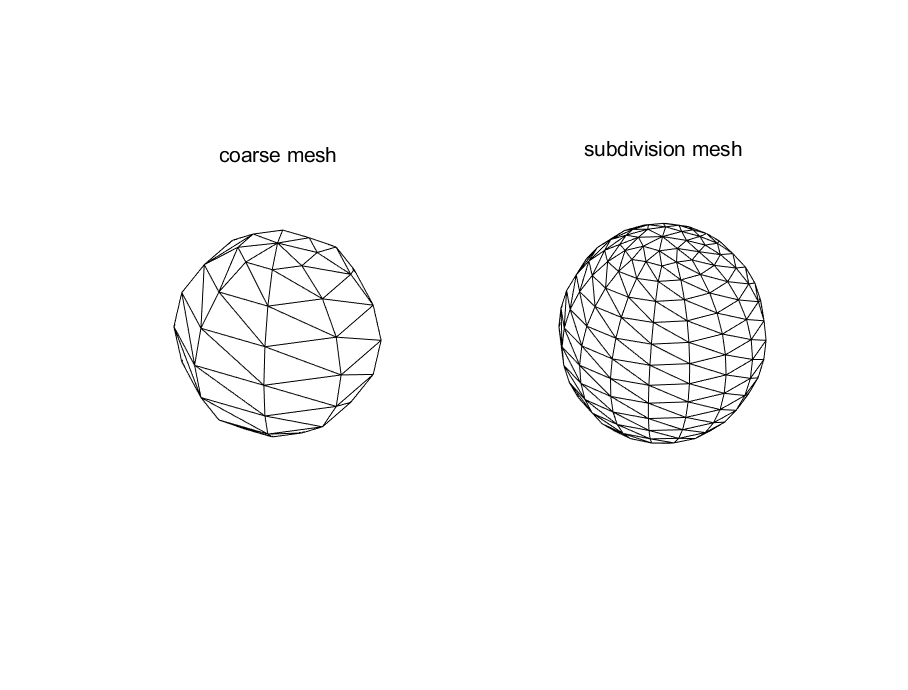
\includegraphics[width=0.5\textwidth]{fig/result_n1.eps}
    \caption{细分一次 ($n=1$) 后的球体网格}
\end{figure}

\subsection{细分次数 $n=2$}

\begin{itemize}
    \item 三角面数量变为原来的 16 倍;
    \item 网格更加均匀;
    \item 球体外观接近光滑曲面.
\end{itemize}

\begin{figure}[ht]
    \centering
    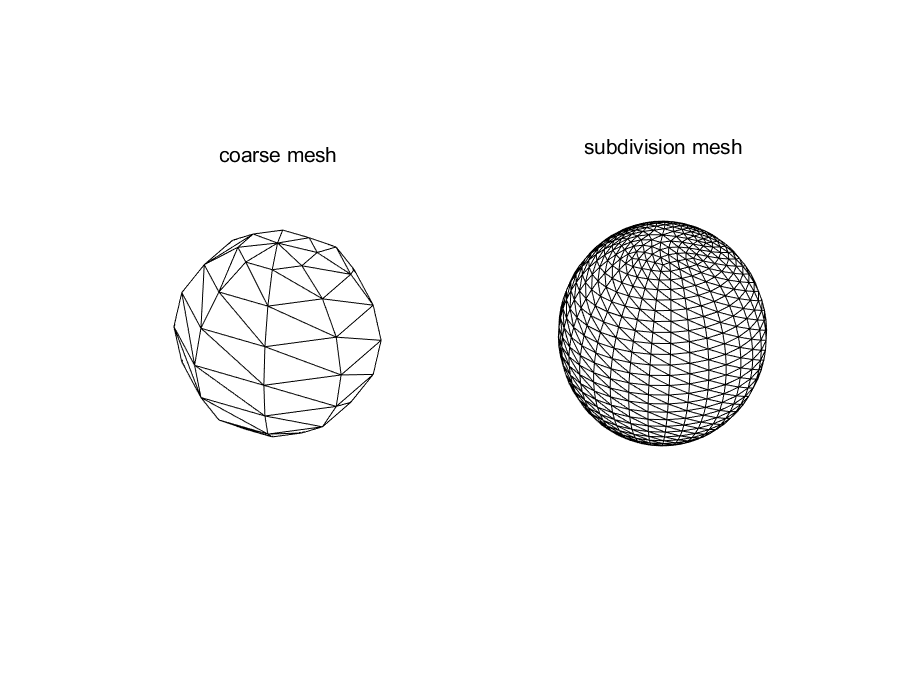
\includegraphics[width=0.5\textwidth]{fig/result_n2.eps}
    \caption{细分两次 ($n=2$) 后的球体网格}
\end{figure}

\subsection{细分次数 $n=5$}

\begin{itemize}
    \item 网格高度稠密;
    \item 已难以分辨三角形结构;
    \item 曲率过渡非常平滑, 逼近真实球面.
\end{itemize}

\begin{figure}[ht]
    \centering
    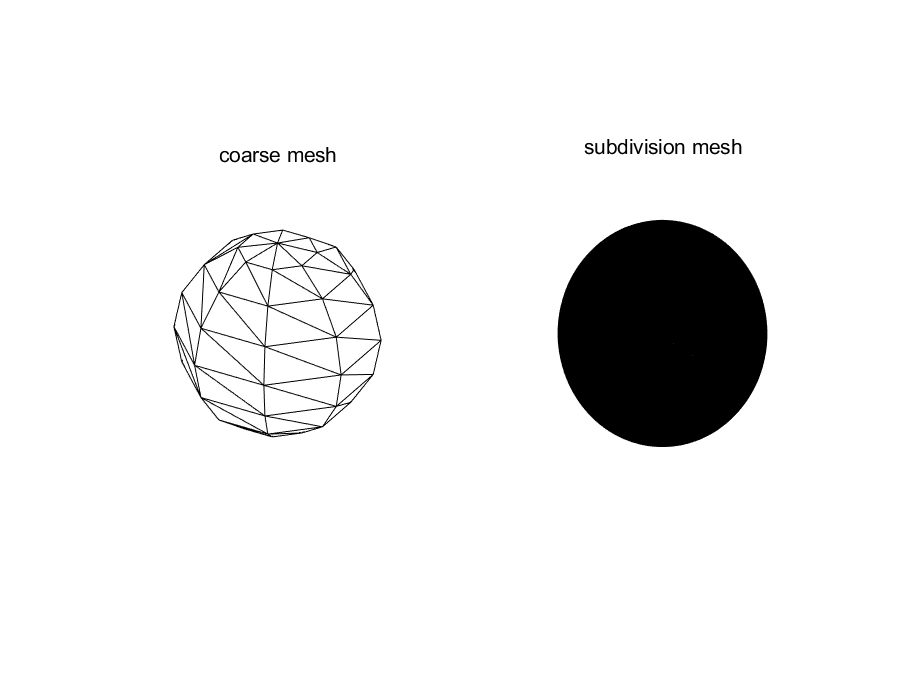
\includegraphics[width=0.5\textwidth]{fig/result_n5.eps}
    \caption{细分五次 ($n=5$) 后的球体网格}
\end{figure}

\clearpage

\section{结果分析}

通过实验可以观察到以下现象:

\begin{itemize}
    \item 随着细分次数增加, 网格顶点数量按指数级增长, 符合 Loop 细分理论;
    \item 球面逐渐变得更加光滑, 面片数量大幅增加;
    \item extraordinary vertices (度不为 6 的点) 区域也趋于光滑, 符合 Loop 的 $C^1$ 性质;
    \item 若使用原框架的绘制代码, 由于绘制使用 \texttt{t} 而非 \texttt{t2}, 导致 ``顶点不增加'' 的错误视觉效果;
    \item 修正后可正确展示细分后的高细节球体表面.
\end{itemize}

实验结果与 Loop 细分的数学理论完全一致, 证明算法实现正确.

\section{总结}

本实验成功实现了 Loop 细分算法的全部步骤, 包括:
\begin{itemize}
    \item 构造边及对顶点关系;
    \item 边界与内部点区分;
    \item Even 与 Odd 顶点位置更新;
    \item 三角面片的四分拓扑更新;
    \item 多级细分的完整 pipeline.
\end{itemize}

实验展示了 Loop 细分的典型效果: 随着细分深度增加, 任意拓扑的网格模型都会逐渐逼近一个光滑曲面. Loop 细分在实际图形学应用中具有重要地位, 是现代渲染和建模系统中常用的平滑处理方法. 本次实验对理解细分曲面理论与实现细节具有重要意义.

\end{document}
